\chapter{Výběr architektury}

\begin{chapterabstract}
	V této kapitole budou popsány možné architektury pro mobilní aplikaci a backend. Cílem je rozdělit aplikaci do různých vrstev, kde každá vrstva bude mít na starosti jednu část zodpovědnosti aplikace. komunikují mezi sebou prostřednictvím pevně definovaného rozhraní. Díky tomu změna implementace jedné vrstvy neovlivní ostatní vrstvy, pokud rozhraní mezi vrstvami zůstane stejné.
\end{chapterabstract}

\section{Mobilní aplikace}

\subsection{Architektura doporučená Googlem}
\label{subsec:architecture-google}
Softwarovou architekturu doporučenou Googlem \cite{android-architecture} ilustruje následující obrázek:

\begin{figure}[h!]
	\centering
	
	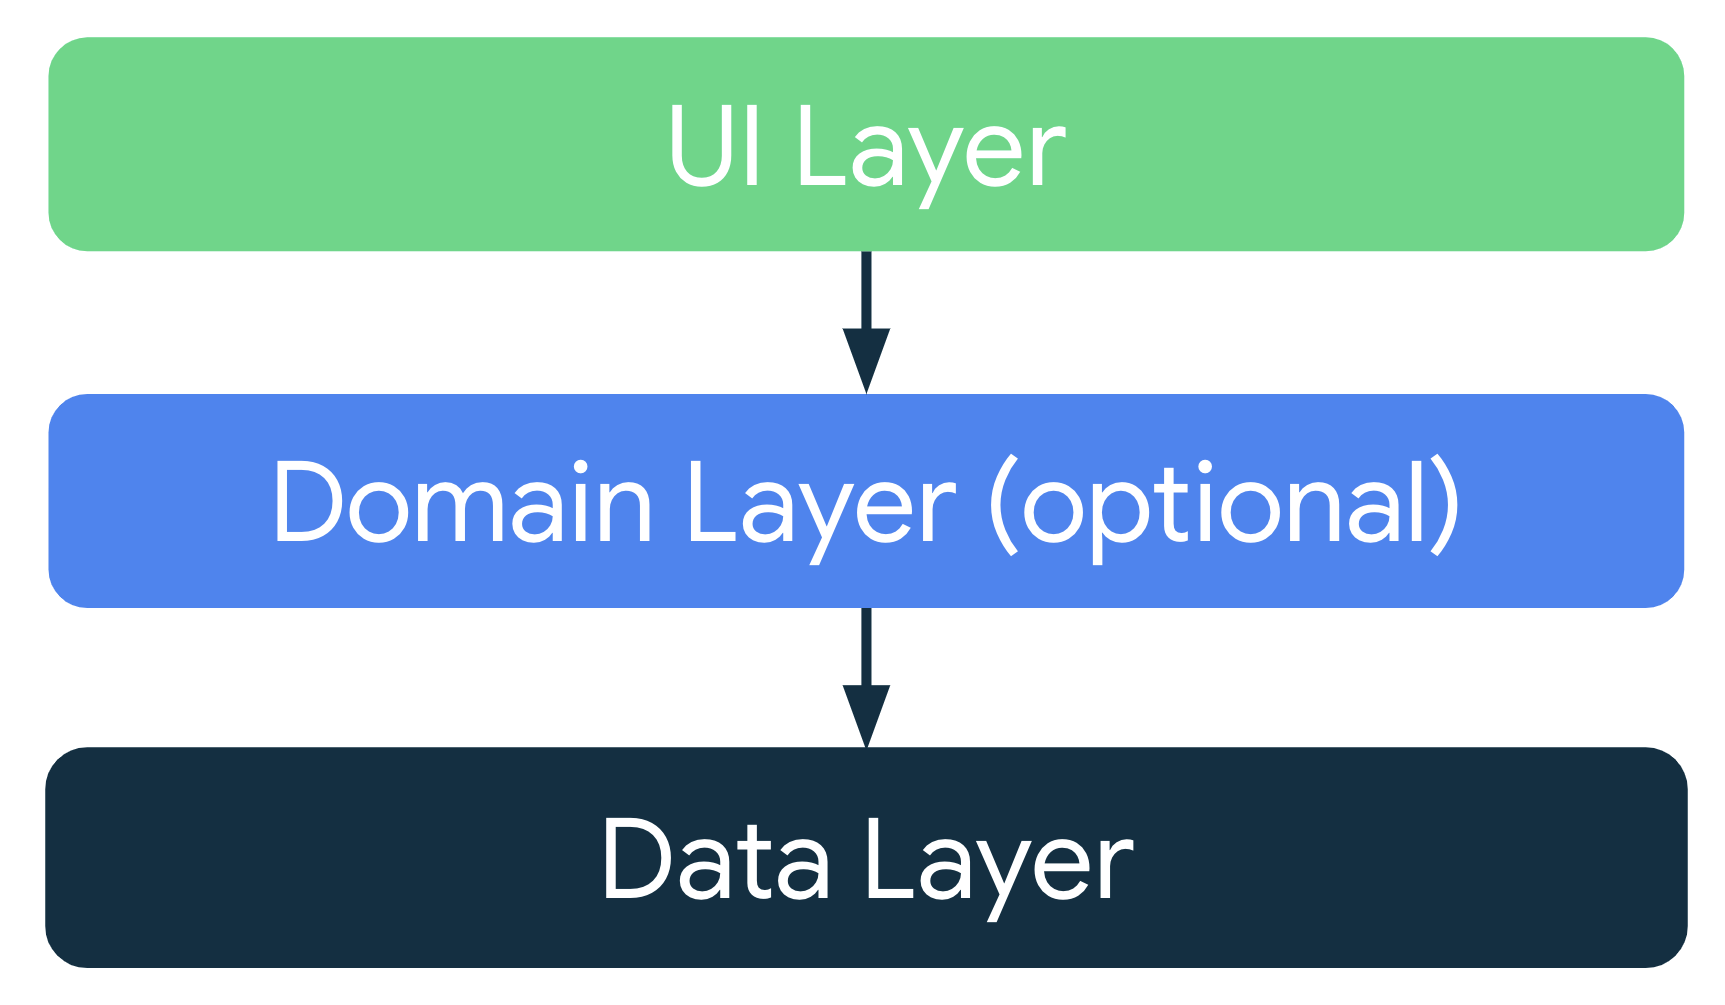
\includegraphics[width=0.5\linewidth]{android-architecture-overall}
	
	\caption{Architektura Android aplikaci \cite{android-architecture}}
	\label{fig:android-architecture-overall}
\end{figure}

\noindent Architektura je rozdělená na UI vrstvu, doménovou vrstvu a datovou vrstvu. UI (také prezentační) vrstva má na starosti zobrazování dat v UI. UI je aktualizováno na základě změn ve stavu UI. Stav UI je měněno prostřednictvím událostí (např. kliknutí na tlačítko) nebo externích vstupů (odpověď ze síťového volání). UI vrstva je složena z UI elementů a držitelů stavu, jak je ilustrováno na následujícím obrázku:

\begin{figure}[H]
	\centering
	
	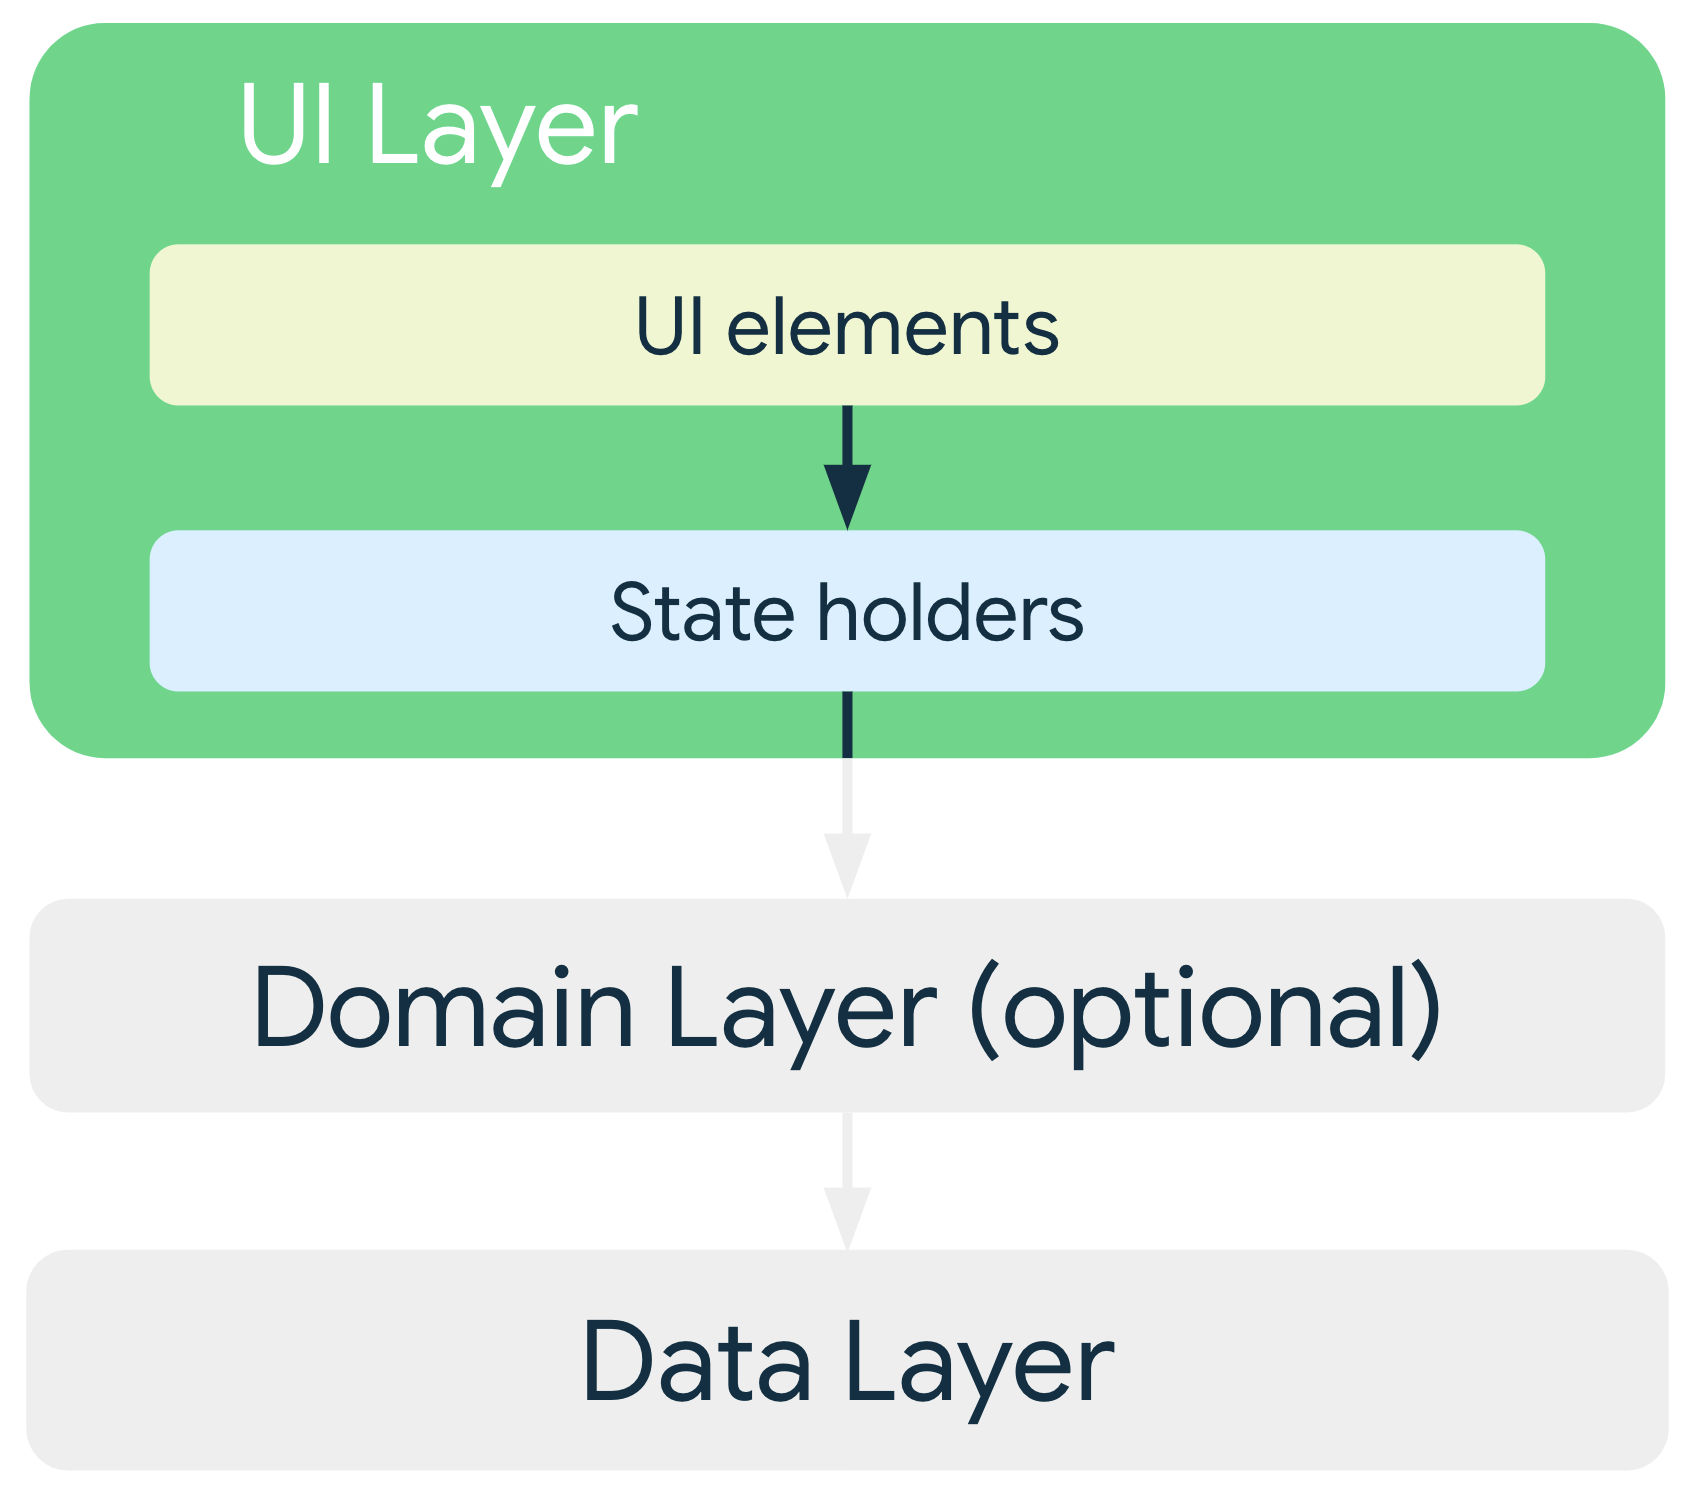
\includegraphics[width=0.5\linewidth]{android-architecture-ui}
	
	\caption{Složení UI vrstvy \cite{android-architecture}}
	\label{fig:android-architecture-ui}
\end{figure}

\noindent UI elementy reprezentují elementy, které jsou vykreslovány na obrazovku. Držitelé stavů mají na starosti správu stavu UI a obsluhu událostí vyvolaných z UI. Změna stavu v držiteli stavu způsobí změnu UI elementů a znovu vykreslení obrazovky. 

Datová vrstva, jak ilustruje následující obrázek, je složena z repozitářů a datových zdrojů. Repozitář vystavuje data pro zbytek aplikace, čímž ho abstrahuje od konkrétního způsobu získávání dat (např. zda jsou data získávána lokálně nebo vzdáleně). Dále repozitář slouží pro centralizaci dat, což je způsob správy dat, kdy je vytvořen jednotný zdroj pravdy, tj. všechna data v aplikaci pochází vždy z tohoto zdroje, ať už přímo nebo nepřímo. Díky tomu jsou všechna data v aplikaci konzistentní. Datový zdroj pak reprezentuje konkrétní zdroj dat, z kterého jsou získávána data. Může to být např. lokální soubor, backend nebo lokální databáze. 

\begin{figure}[H]
	\centering
	
	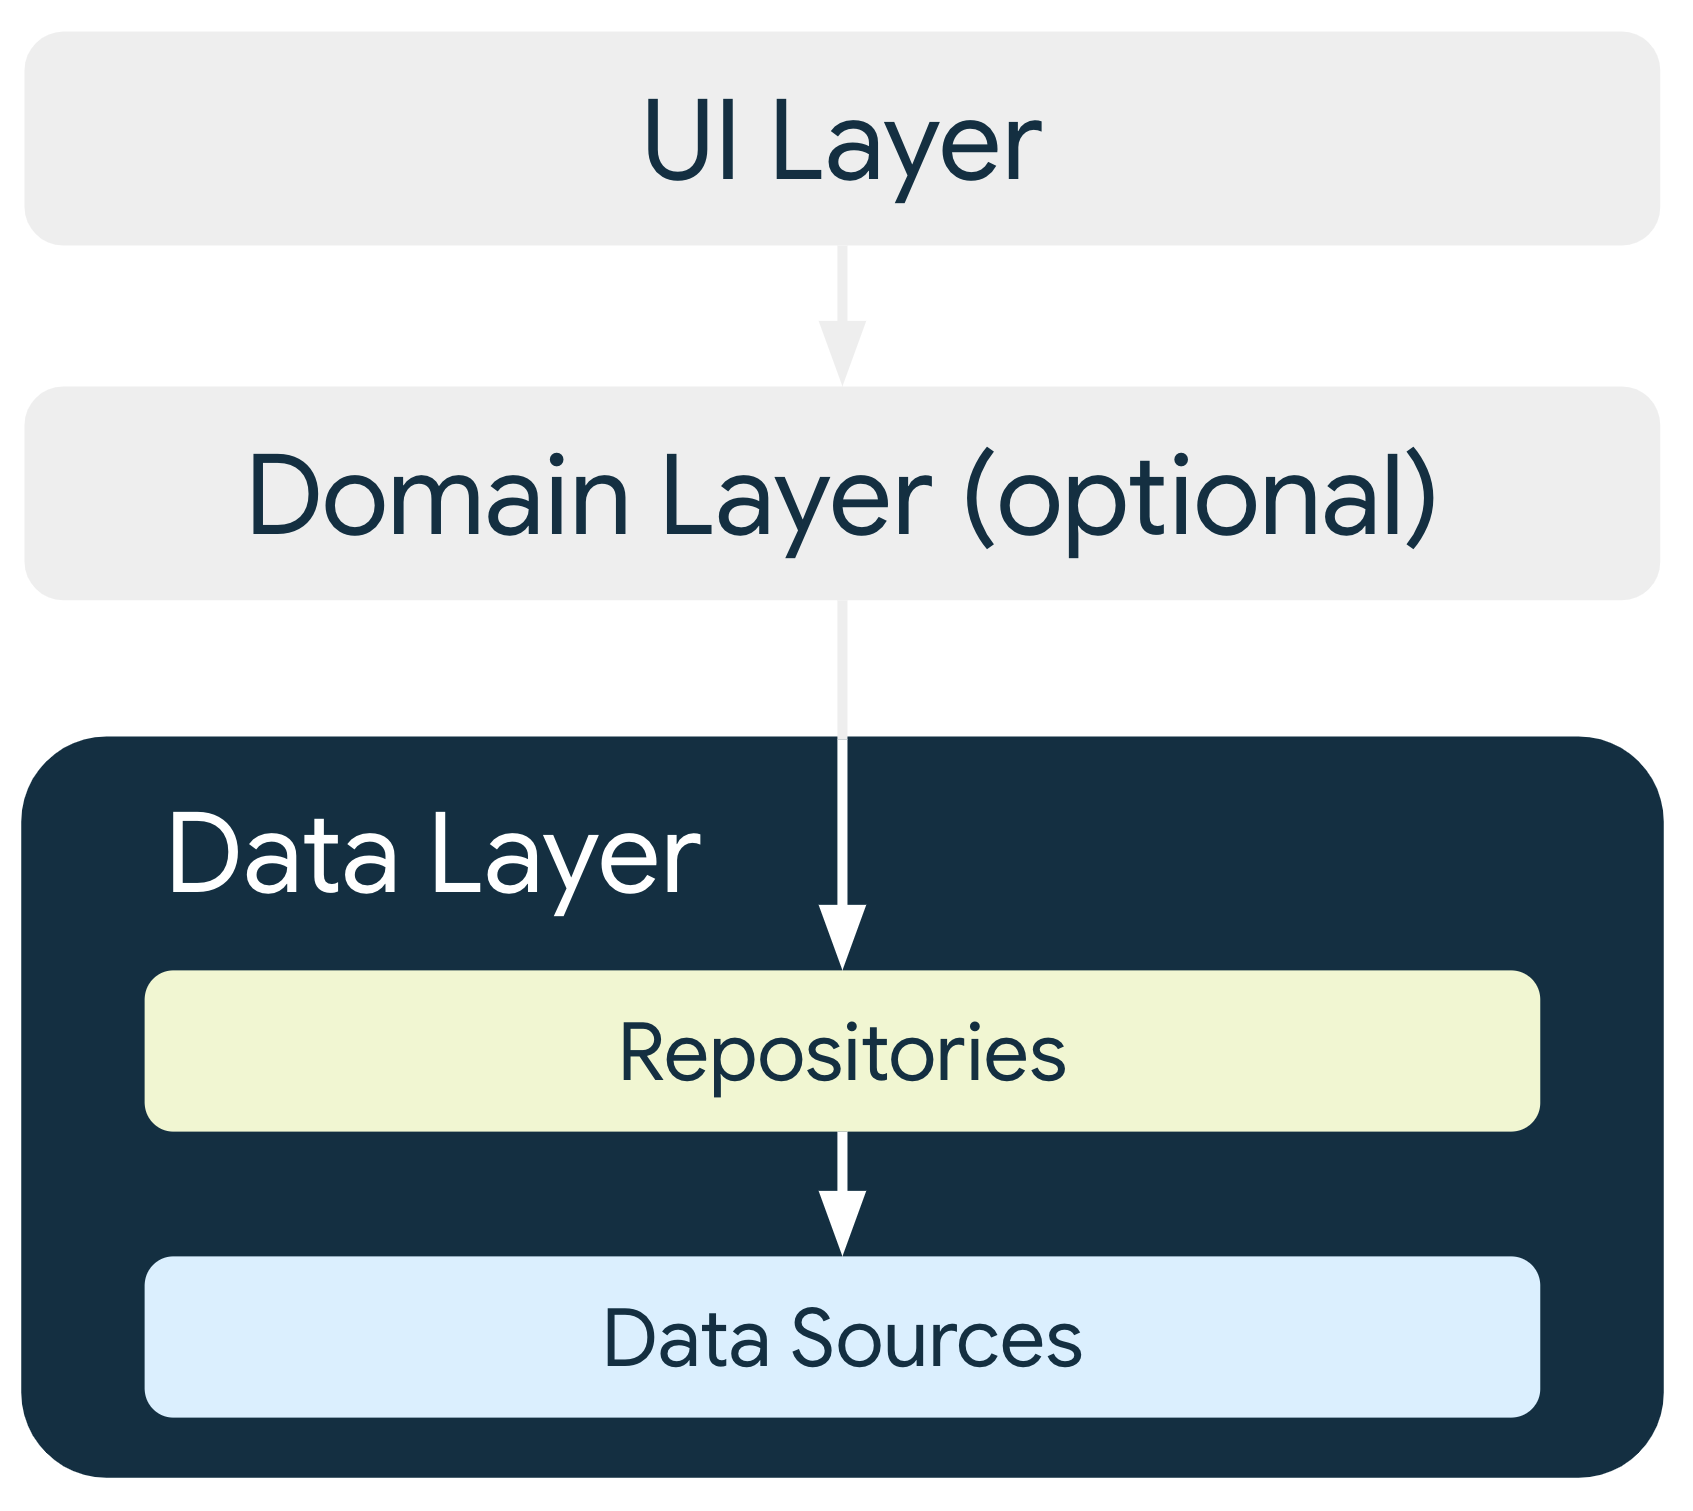
\includegraphics[width=0.5\linewidth]{android-architecture-data}
	
	\caption{Složení datové vrstvy \cite{android-architecture}}
	\label{fig:android-architecture-data}
\end{figure}

\noindent Doménová vrstva má na starosti zapouzdření business logiky. Díky tomu je business logika přepoužitelná ve více držitelích stavů, pokud jich používáme několik. Třídám v této vrstvě říkáme \textit{use cases} nebo \textit{interactors}.

\subsection{Zhodnocení}
Architektura doporučená Googlem má následující výhody:

\begin{itemize}
	\item \textbf{Oddělení zodpovědnosti} -- Rozdělení aplikace do vrstev zlepšuje udržitelnost aplikace.  Vrstvy mají mezi sebou pevně definované rozhraní. Změna implementace jedné vrstvy bude mít minimální vliv na ostatní vrstvy.

	\item \textbf{Řízení UI podle stavu dat} -- Uživatelské rozhraní automaticky reaguje na změnu stavu dat UI. 

	\item \textbf{Jednotný zdroj pravdy} -- Zajišťuje konzistenci dat.

	\item \textbf{Jednosměrný tok dat} -- Data putují pouze zeshora dolu (např. z datového zdroje k repozitáři, z repozitáře k držiteli stavu). Události putují pouze zezdola nahoru (např. z UI elementů k držitěli stavu, z držitele stavu k repozitáři). Díky tomu je fungování aplikace predikovatelné a snadno debugovatelné.

	\item \textbf{Je doporučený Googlem} -- Architektura je díky tomu obecně známá. Když by na této práce začal pracovat jiný Android vývojář, vyznal by se díky této architektuře v kódu lépe.
\end{itemize}

\noindent Z těchto důvodů byla pro implementaci mobilní aplikace vybrána tato architektura. 

\section{Backend}

\subsection{5-vrstvá architektura}
5-vrstvá architektura \cite{5-tier} rozděluje aplikaci do následujících vrstev:


\begin{itemize}
	\item \textbf{Prezentační} -- Má na starosti prezentaci dat uživatelovi a obsluhu událostí. Data získává \linebreak z aplikační vrstvy.
	
	\item \textbf{Aplikační} -- Funguje jako prostředník mezi prezentační a businessovou vrstvou. Má na starosti aplikační logiku a řídí tok dat mezi různými vrstvami. Implementuje mimo jiné autentizaci, autorizaci a validaci dat.
	
	\item \textbf{Businessová} -- Obsahuje businessovou logiku aplikace. Definuje operace, které mohou být prováděny na datech, a implementuje businessové procesy. Komunikuje s perzistentní vrstvou pro ukládání a získání dat.	
	
	\item \textbf{Perzistentní} -- Tato vrstva má na starosti ukládání a získávání dat z databáze. Funguje jako abstraktní rozhraní pro bussinessovou vrstvu pro přístup k datům. Data ukládá a získává prostřednictvím komunikace s API databáze v databázové vrstvě.
	
	\item \textbf{Databázová} -- Má na starosti ukládání dat. Může být implementována např. pomocí relační databáze. Poskytuje data perzistentní vrstvě.
	
\end{itemize}

\noindent U větších projektů lze projekt také rozdělit podle funkcionalit (např. funkcionalita pro poskytování informací o hlasování a funkcionalita pro poskytování informací o poslancích) a v rámci těchto funkcionalit použít 5-vrstvou architekturu.

\subsection{Architektura mikroslužeb}
Architektura mikroslužeb je architektonický styl, který rozděluje aplikaci do služeb, což jsou komponenty s následujícími vlastnostmi:

\begin{itemize}
	\item \textbf{Samostatně nasaditelné} -- Každou službu lze nasadit zvlášť od ostatních služeb.

	\item \textbf{Volně propojené} -- Služby komunikují mezi sebou prostřednictvím API, a nejsou tedy závislé na implementaci druhého.
	
	\item \textbf{Rozdělené podle domény} -- Každá služba má na starosti určitou doménu v byznysu. \linebreak Např. jedna služba má na starosti účetnictví a jiná má na starosti objednávky.
	
	\item \textbf{Vývoj v několika týmech} -- Jednotlivé služby lze vyvíjet nezávisle na ostatních \linebreak službách, dokud je zachováno API mezi nima.
	
	\item \textbf{Dobře testovatelné a udržitelné} -- Každou službu lze testovat a udržovat zvlášť od ostatních služeb.
\end{itemize}

\subsection{Zhodnocení}
5-vrstvá architektura je pro účely této práce dostačující. Prezentační vrstva bude použita pro vytvoření endpointů REST API. Aplikační vrstva nebude pro jednoduchost \linebreak implementována, a místo toho budou její zodpovědnosti implementovány v rámci businessové vrstvy. Businessová vrstva bude sloužit pro abstrahování prezentační vrstvy od perzistentní vrstvy. Zároveň bude sloužit pro validaci dat. Backend nebude mít složitou business \linebreak logiku, bude pouze zpracovávat data z webu PSP a vystavovat je prostřednictvím REST API. Perzistentní vrstva bude použita pro abstrakci businessové vrstvy od databázové. To usnadní práce s databází. V rámci databázové vrstvy budou ukládáná data. Chybí tu však vrstva pro pravidelnou aktualizaci databáze. Backend bude totiž pravidelně stahovat data z webu PSP a aktualizovat databázi. K této architektuře tedy bude navíc přidána vrstva pro synchronizaci databáze se zdrojovými daty na web PSP.

Architektura mikroslužeb se hodí pro velké projekty, kde je předpokládáno, že budou často přicházet nové požadavky o nové funkcionality v různých částech backendu. V takovém případě je dobré backend rozdělit do nezávislých částí a ty vyjíjet, testovat, nasazovat a udržovat odděleně ve více týmech. Nevýhodou je větší komplexita projektu. Pro účely této práce toto rozdělení není potřeba, jelikož požadavky jsou předem dané a nepředpokládá se, že se budou \linebreak v budoucnu měnit. Všechny části backendu tedy budou mezi sebou komunikovat prostřednictvím programového rozhraní, nikoliv API.


